\documentclass[14pt]{extreport}
\usepackage{gost}

\begin{document}

\pagestyle{empty}
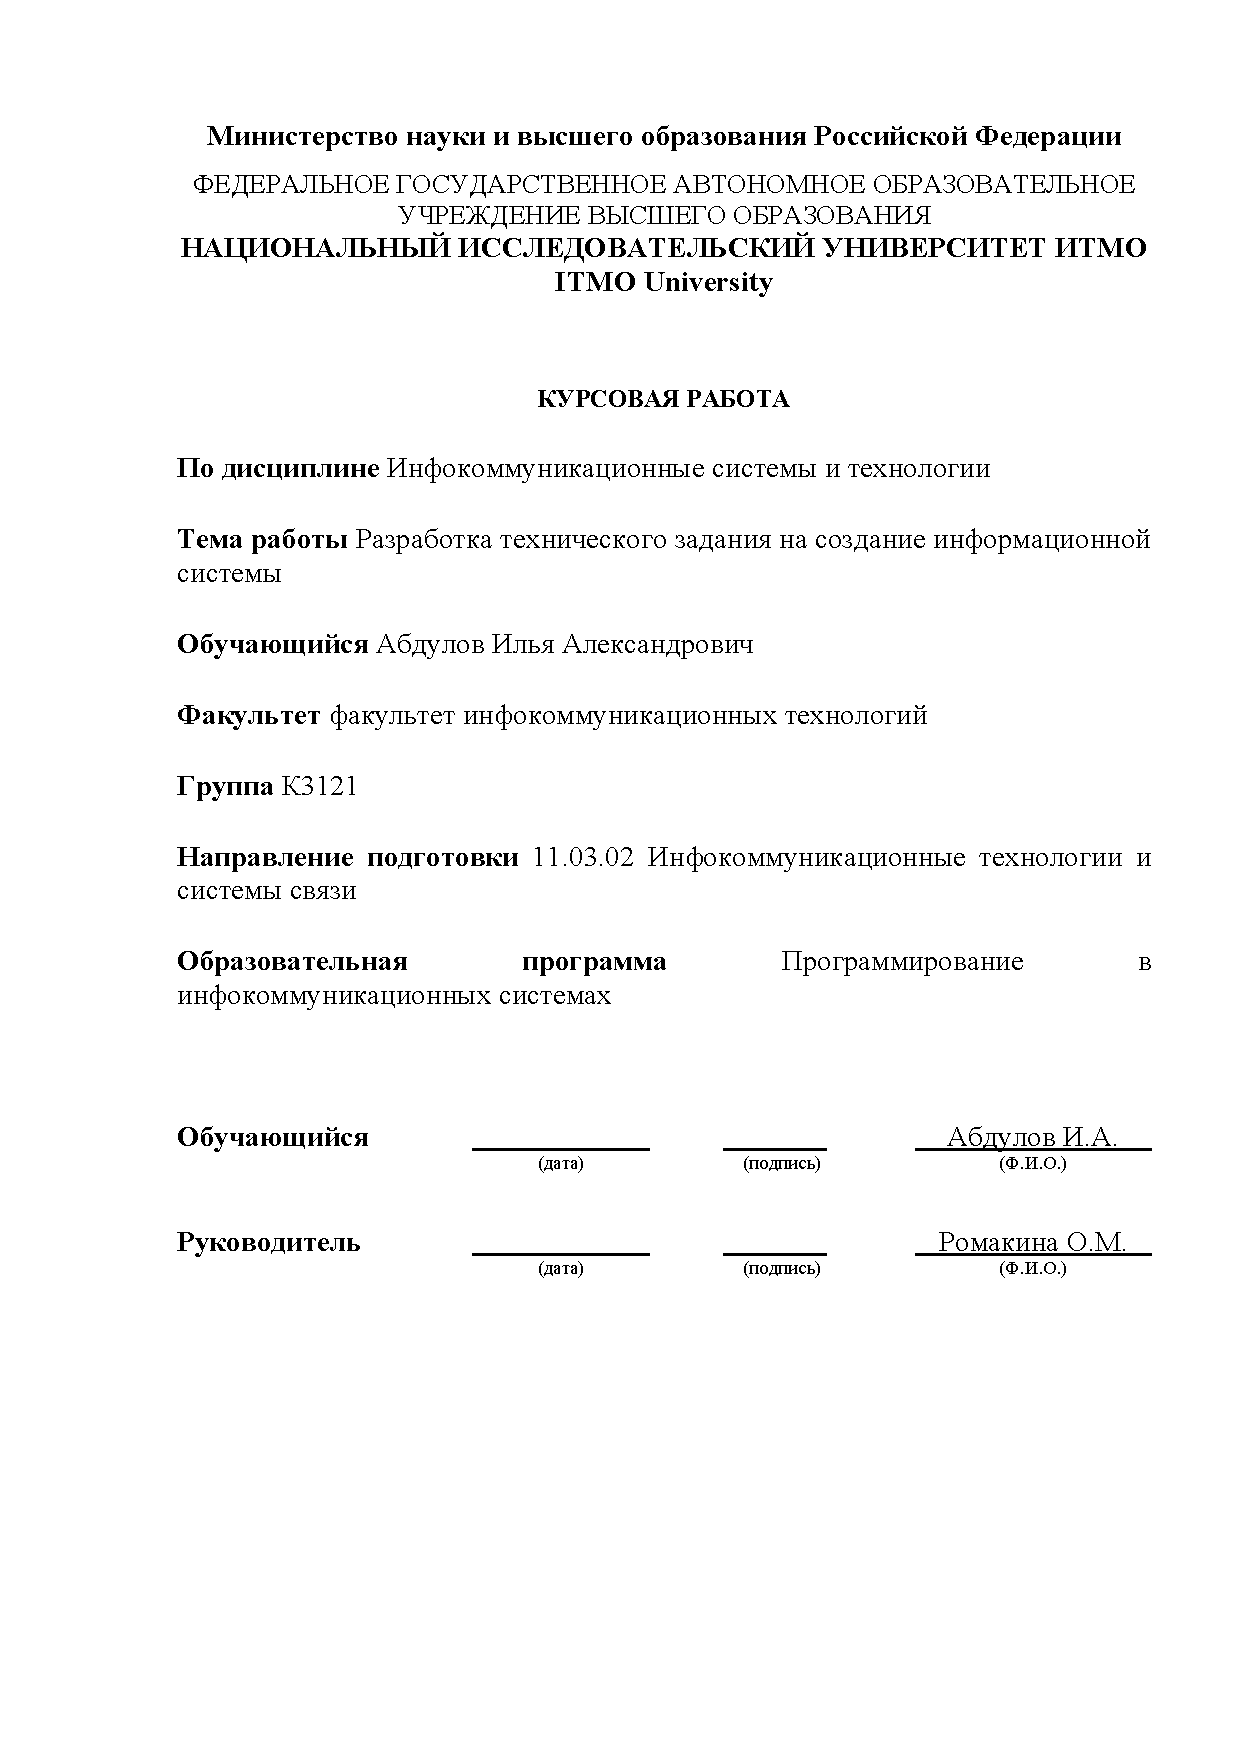
\includepdf{titulCourse.pdf}
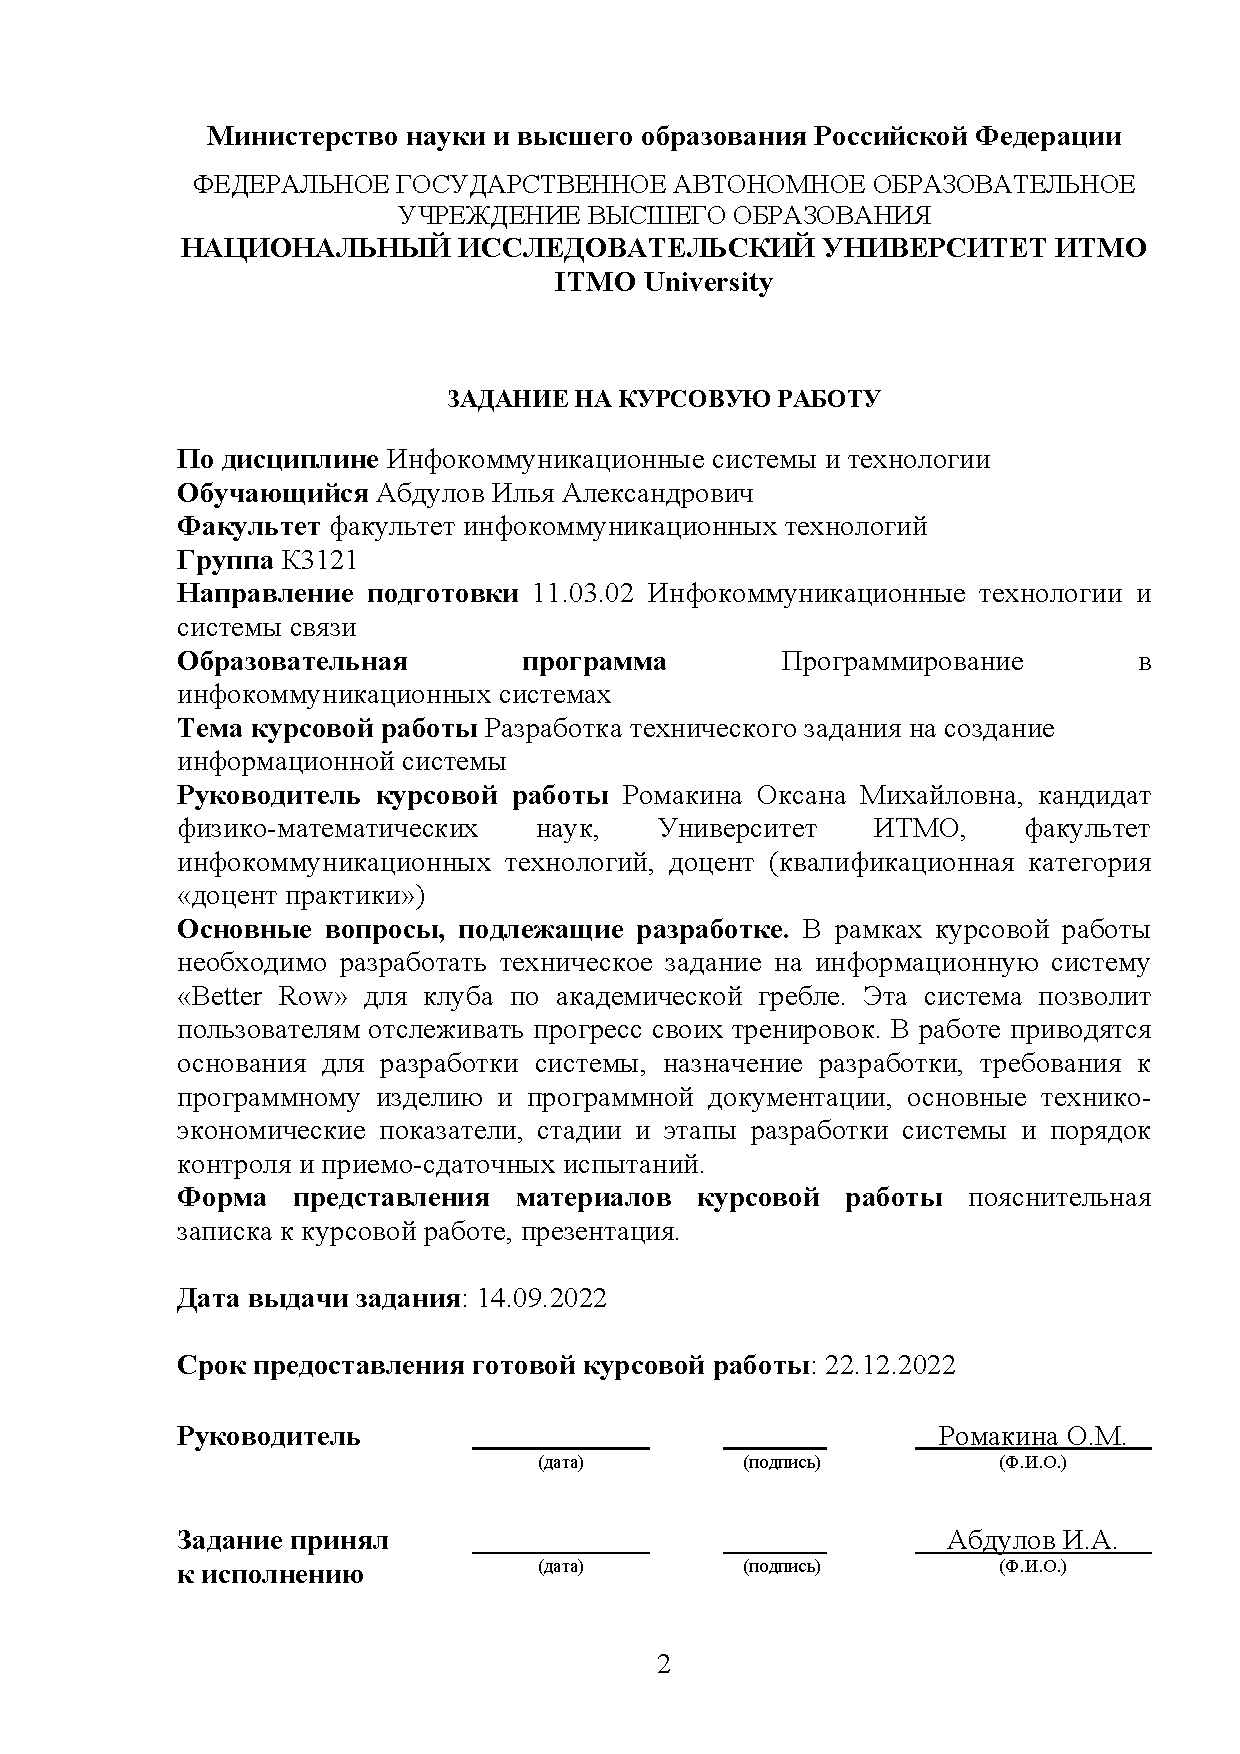
\includepdf{taskCourse.pdf}
\pagestyle{plain}

\begin{abstract}

\begin{minipage}{0.4\textwidth}
  
\end{minipage}
\hfill
\begin{minipage}{0.4\textwidth}
\begin{frame}

Абдулов И.А. Разработка технического задания на создание информационной системы. – Санкт-Петербург: ИТМО, 2022, 41 с., 19 ил., библиогр. список – 14 наим.

\end{frame}
\end{minipage}

\begin{figure} [H]
\end{figure}

Объектом разработки является техническое задание на создание информационной системы.

Целью курсовой работы на основе проведенного анализа является разработка технического задание на мобильное приложение «Better Row» для университетского клуба по академической гребле.

В курсовой работе приводятся основания для разработки информационной системы, назначение разработки, требования к программному изделию и программной документации, стадии и этапы разработки системы и порядок контроля и приемо-сдаточных испытаний мобильного приложения «Better Row».

Результаты курсовой работы имеют практическую значимость и могут применяться в непосредственной разработке мобильного приложения для университетского клуба по академической гребле.
\end{abstract}

\tableofcontents

\intro

Тема исследования курсовой работы является актуальной, потому что спортивная деятельность активно развивается и поощряется в университете ИТМО и других, в связи с чем разработка современного программного обеспечения для спортсменов является частью развития деятельности спортивных клубов и секций.

В настоящее время существует лишь небольшое число мобильных приложений или иных информационных систем, которые удовлетворяют потребностям спортсменам. Большинство приложений не нашли применения со стороны спортсменов, поэтому требуется программное обеспечение, которое будет постоянно дорабатываться и улучшаться, основываясь на отзывах пользователей, чтобы им было удобно и легко использовать информационную систему на регулярной основе.

Приложение «Better Row» найдет применение среди спортивных клубов и удовлетворит потребности спортсменов в программном обеспечении. Эта информационная система представляет из себя приложение, куда пользователь заносит данные своих тренировок, чтобы приложение показывало и сохраняло текущие показатели и прогресс. Использование приложения придаст тренировкам осознанности, что поможет в достижении лучшего результата.

Целью данной работы является разработка технического задания на мобильное приложение.

В связи с поставленной целью необходимо решить следующие задачи:

\begin{enumerate}

\item Описать предметную область и необходимые функции будущей ИС;

\item Описать основную идею предлагаемой ИС или будущего мобильного приложения. Описание идеи будущей ИС включает: название, назначение, основных пользователей системы, планируемый набор функций для каждого из будущих пользователей, прототип интерфейса будущей системы, обзор аналогов на рынке и обоснование необходимости разработки планируемой системы;

\item Описать основных пользователей будущего мобильного приложения, используя диаграммы UML;

\item Построить функциональную модель в стандарте IDEF0, которая включает 3 уровня декомпозиции и предусматривает обратные связи между работами по входу или управлению;

\item Построить диаграммы DFD, модели IDEF3 с двумя уровнями декомпозиции;

\item Создать техническое задание на разработку мобильного приложения.

\end{enumerate}

\chapter{Анализ предметной области}

\section{Описание предметной области и необходимых функций будущей ИС, подлежащих реализации}

Приложение предназначено для развития спортивной деятельности в университете ИТМО, оно предназначено для клуба по академической гребли. Функциональные возможности приложения должны позволять пользователю сохранять данные о тренировке и всесторонне анализировать их для удобства отслеживания прогресса.

Основными пользователями системы будут являться любители академической гребли и участники студенческой гребной лиги России.

\subsection{Название}

Название приложения {Better Row}\footnote{Лучше Греби – дословный перевод с английского} отражает цель приложения: помочь пользователю улучшить свои показатели и результаты в таком соревновательном виде спорта, как академическая гребля.

\subsection{Назначение}

Назначение приложения: позволить пользователю сохранять данные о своих тренировках на гребном тренажере, чтобы в дальнейшем иметь возможность их просмотреть. Приложение поможет следить за своими показателями тренировок, видеть свой прогресс и иметь возможность поделиться своими результатами с тренером по сети Интернет.

\subsection{Основные пользователи}

Основными пользователями системы будут являться любители академической гребли и участники студенческой гребной лиги России.

\subsection{Планируемый набор функций}

Для каждого из будущих пользователей планируется реализовать три вкладки в главном меню: результаты и статистика, расписание тренировок, настройки приложения.

Во вкладке результатов пользователь сможет перемещаться по дням и либо просматривать результаты тренировки в этот день, либо добавлять информацию о тренировке. При добавлении тренировки пользователь вводит дистанцию, время, темп заплыва на гребном тренажере – обязательные показатели, а также пульс после заплыва – опциональную характеристику для ввода. При просмотре тренировок, которые уже были добавлены, к введённым показателям автоматически добавляется рассчитанная приложением средняя скорость заплыва. Кроме того, реализованы функции просмотра изменения результата по сравнению с прошлыми тренировками.

Во вкладке расписания тренировок будут указанные дни недели, в которые проходят тренировки, время и место занятий секции. Если расписание тренировок поменяется, то, используя функцию, его можно будет изменить в той же вкладке.

Во вкладке настроек приложения будут функции смены аккаунта пользователя и сброса данных о всех тренировках.

\subsection{Прототип интерфейса}

Прототип интерфейса реализован в онлайн-инструменте Figma:

\begin{figure}[H]
\centerline{\includegraphics[width=0.75\linewidth]{iphone 8 - 3.pdf}}
\caption{Главная страница}
\label{fig11}
\end{figure}

\begin{figure}[H]
\centerline{\includegraphics[width=0.75\linewidth]{iphone 8 - 1.pdf}}
\caption{Страница результатов и статистики, тренировка 25 октября}
\label{fig12}
\end{figure}

\begin{figure}[H]
\centerline{\includegraphics[width=0.75\linewidth]{iphone 8 - 2.pdf}}
\caption{Страница результатов и статистики, создание тренировки 28 октября}
\label{fig13}
\end{figure}

\begin{figure}[H]
\centerline{\includegraphics[width=0.75\linewidth]{iphone 8 - 4.pdf}}
\caption{Страница расписания}
\label{fig14}
\end{figure}


\section{Обзор аналогов, представленных на рынке}

Среди аналогов, представленных на рынке приложений можно выделить:

\begin{enumerate}
\item Watersports Tracker. Приложение, которое предоставляет статистику о тренировке на воде, отслеживая геолокацию смартфона. Приложение бесплатно для скачивания. Пользователи всех водных видов спорта могут воспользоваться данным приложением, чтобы отследить основные показатели такие, как скорость, время, дистанцию, а также маршрут своего заплыва. Плюсы: красивый дизайн, ничего лишнего. Минусы: пользователям требуется приобрести подписку. Вывод: система удобна для пользования на открытом воздухе, но требует покупки подписки.
\begin{figure}[H]
\centerline{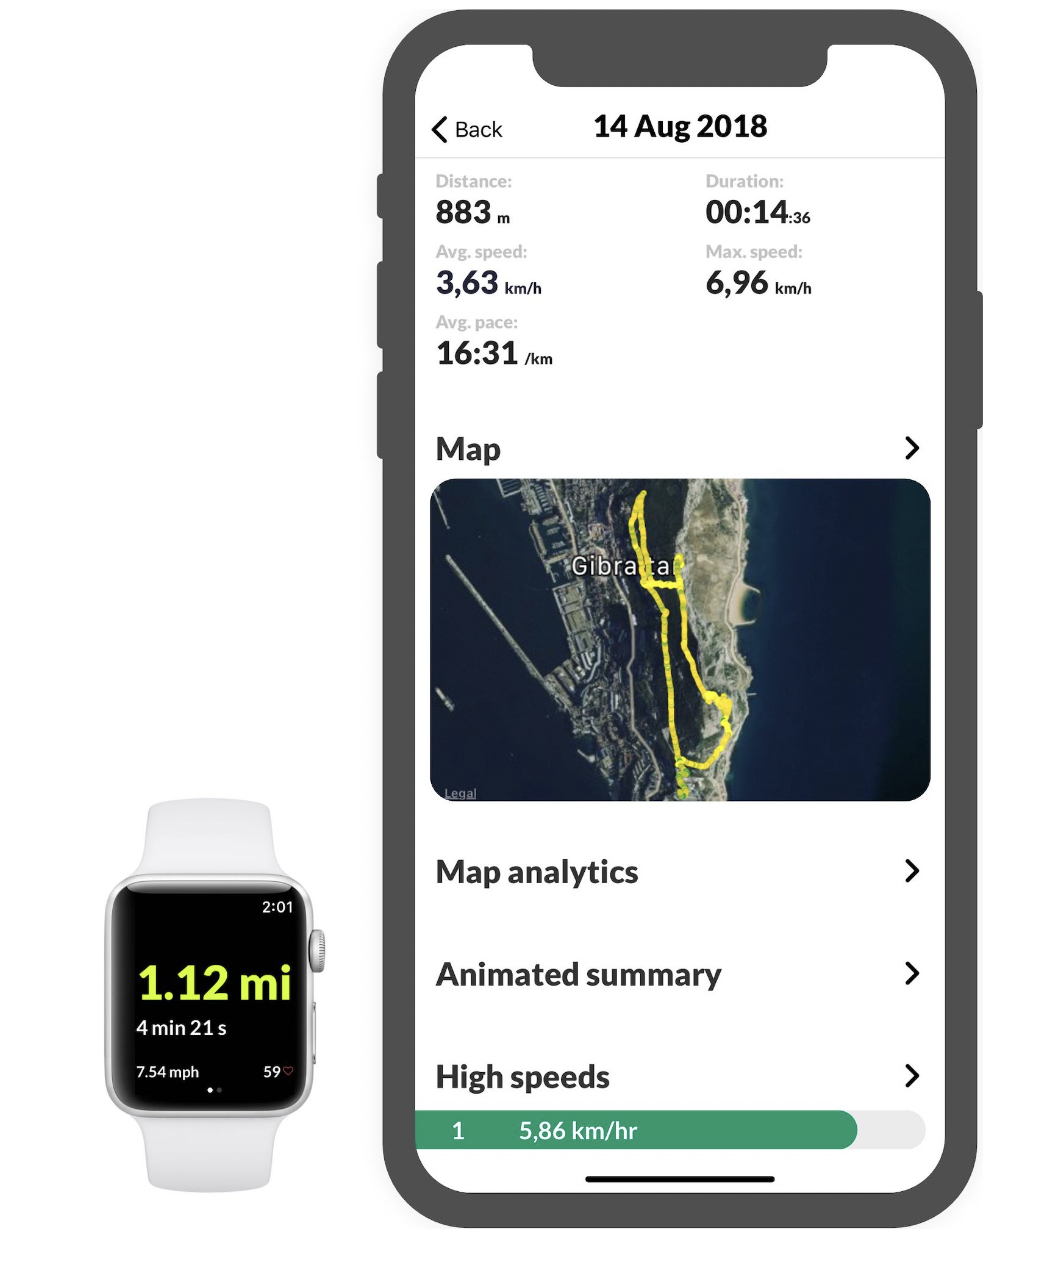
\includegraphics[width=0.7\linewidth]{Watersports Tracker}}
\caption{Watersports Tracker}
\label{fig14}
\end{figure}
\item RowingCoach 4.0. Приложение предоставляет статистику и показатели тренировки, отслеживая геолокацию пользователя. Приложение бесплатно для скачивания. Гребцам предоставляется большой список показателей заплыва, с возможностью посмотреть промежуточные результаты на участке пути, отображается маршрут на карте. Плюсы: подробное, с широким функционалом. Минусы: перестало поддерживаться разработчиком. Вывод: приложение предоставляет все данные о тренировке на воде, но уже несколько лет не обновляется разработчиком.
\begin{figure}[H]
\centerline{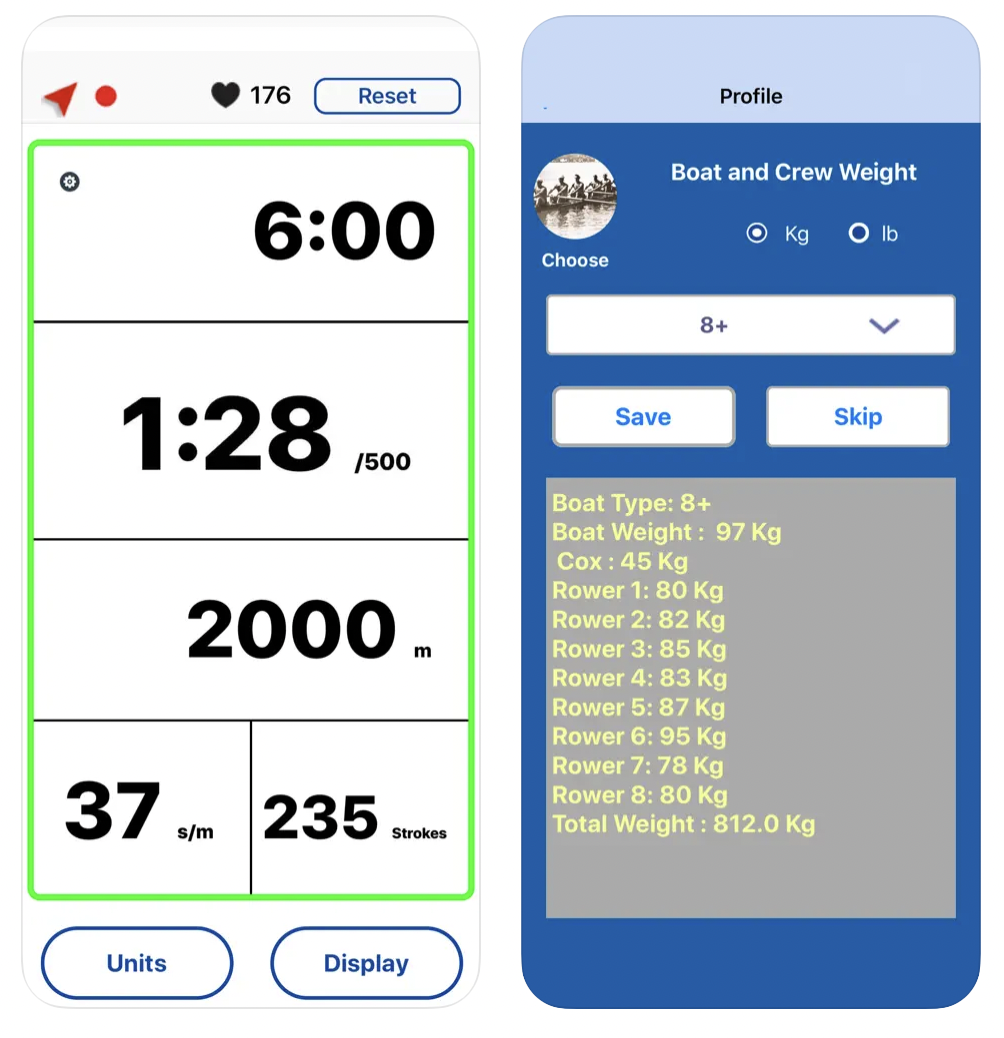
\includegraphics[width=0.7\linewidth]{RowingCoach}}
\caption{RowingCoach 4.0}
\label{fig14}
\end{figure}
\end{enumerate}

\section{Обоснование необходимости разработки}

Все доступные в магазинах приложений аналоги разрабатываемой системы удобны в использовании, потому что автоматически следят за скоростью и показателями на воде. Но аналоги не дают возможности отслеживать показатели тренировок в спортивном зале на гребном тренажере. Приложения берут данные о движении и геолокации смартфона, используя навигацию. Информационная система «Better Row» необходима, потому что нацелена на тренировки в закрытом помещении, сухом зале гребли. Все показатели тренировки пользователь заносит в ИС самостоятельно, чтобы увидеть прогресс или упадок показателей своих тренировок.

\section{Разработка модели прецедентов и диаграмм активности для типовых сценариев работы системы}

\subsection{UML диаграммы}

\begin{figure}[H]
\centerline{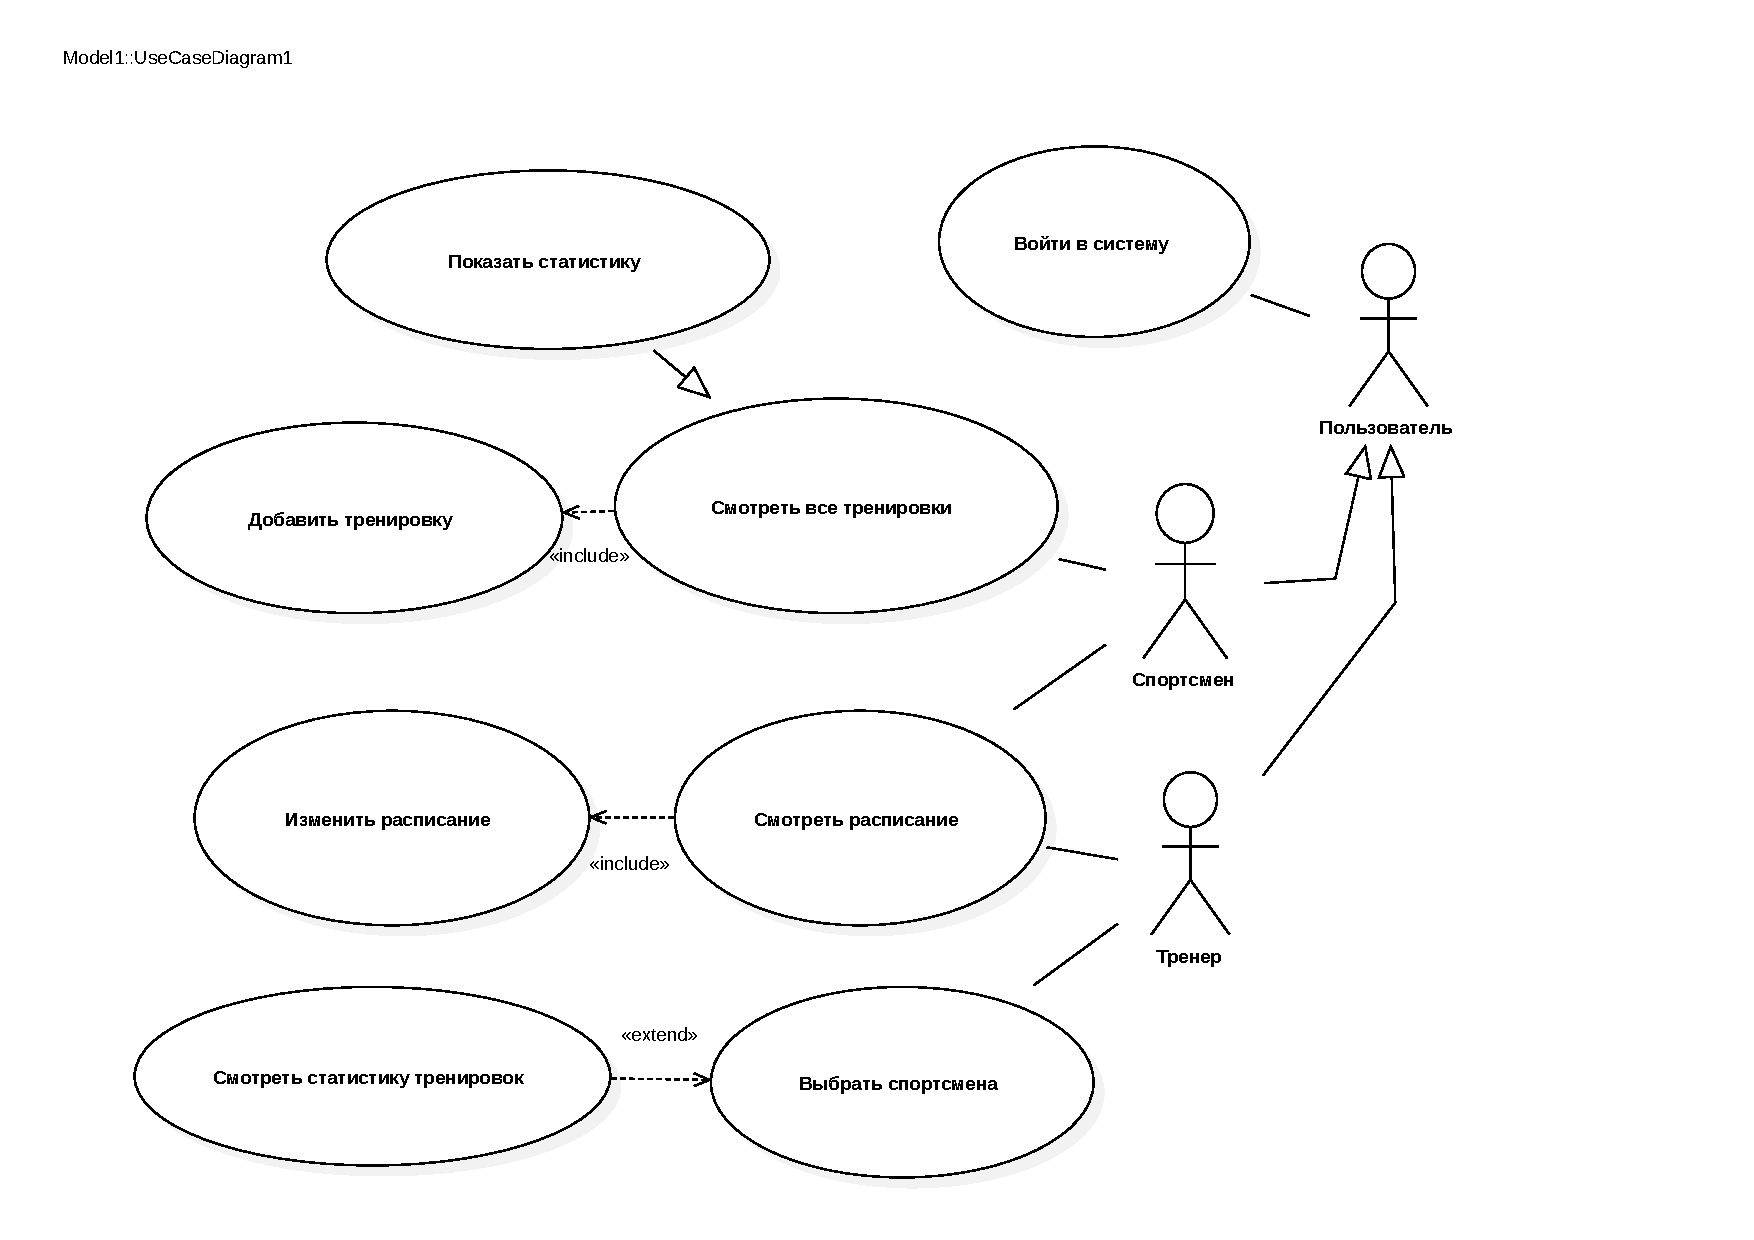
\includegraphics[width=1.2\linewidth]{UseCaseDiagram.pdf}}
\caption{Диаграмма вариантов использования}
\label{fig11}
\end{figure}

\begin{figure}[H]
\centerline{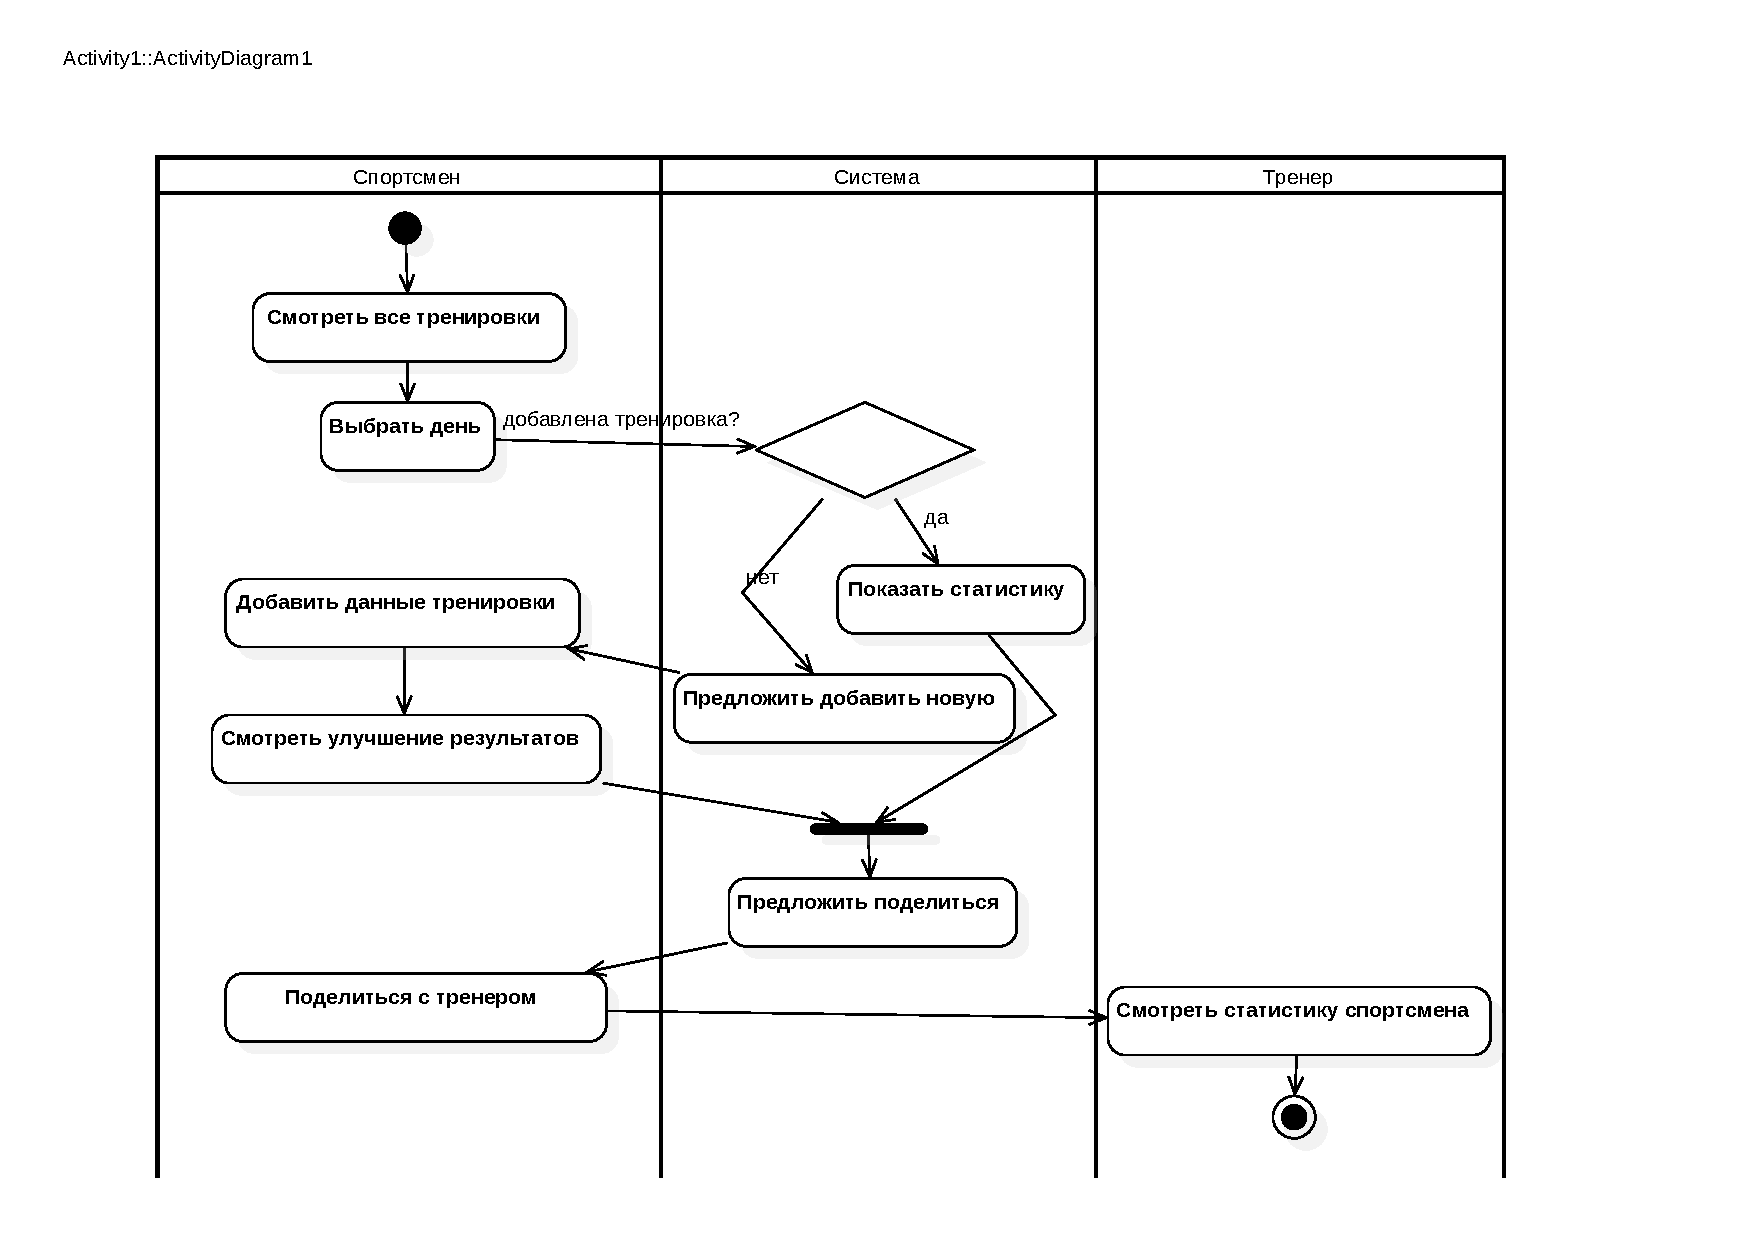
\includegraphics[width=1.2\linewidth]{ActivityDiagram.pdf}}
\caption{Диаграмма активности для ключевого прецедента}
\label{fig12}
\end{figure}

\begin{figure}[H]
\centerline{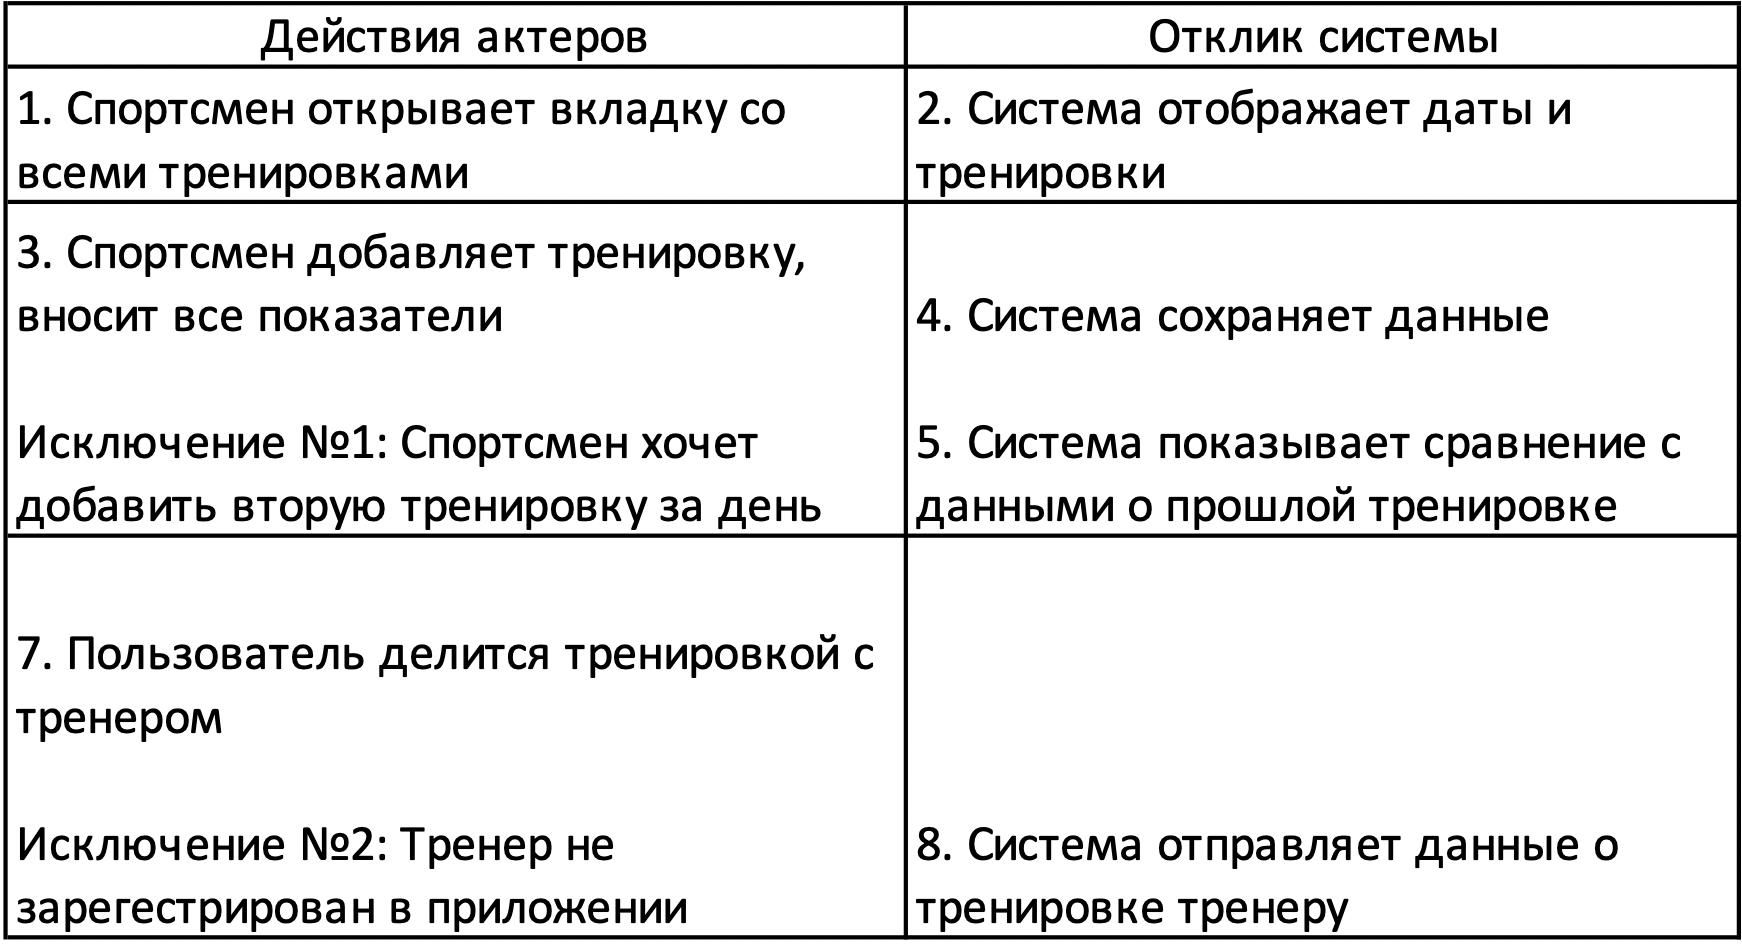
\includegraphics[width=1\linewidth]{Альтернативные потоки.png}}
\caption{Типичный ход события сценария выполнения варианта использования}
\label{fig13}
\end{figure}

\begin{figure}[H]
\centerline{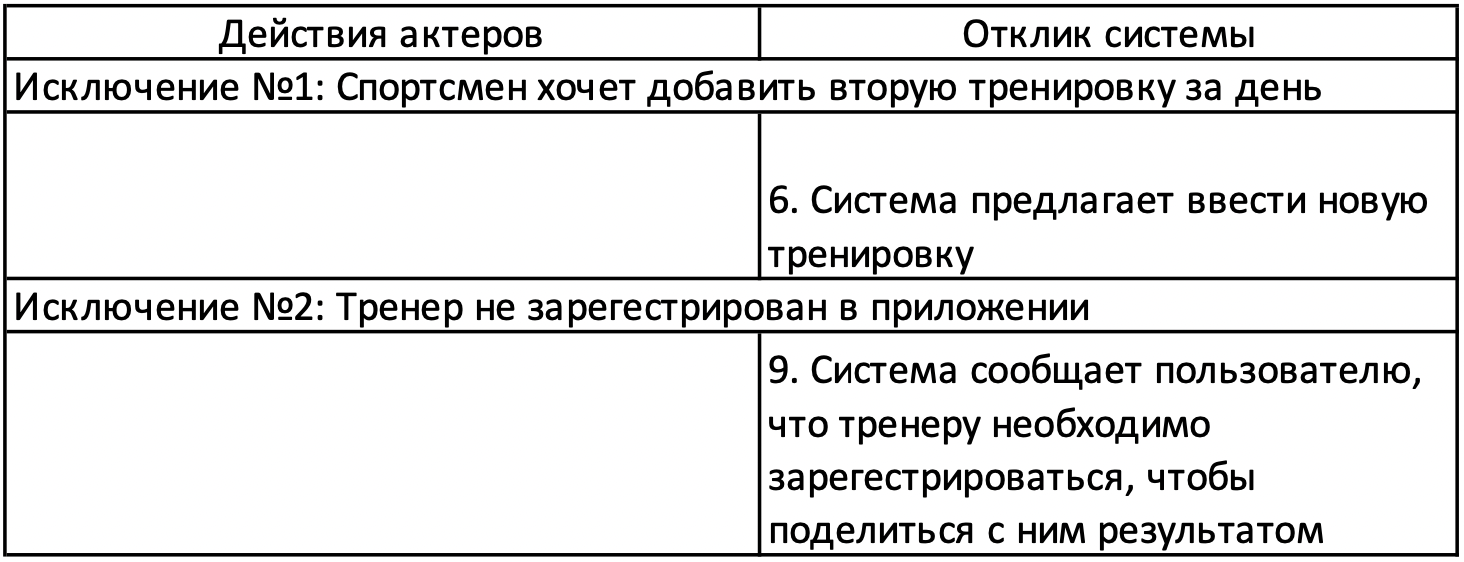
\includegraphics[width=1\linewidth]{Исключения.png}}
\caption{Исключения сценария выполнения варианта использования}
\label{fig14}
\end{figure}

\section{Разработка диаграмм IDEF0, DFD, IDEF3 для будущей системы}

\subsection{Методология IDEF0}

\begin{figure}[H]
\centerline{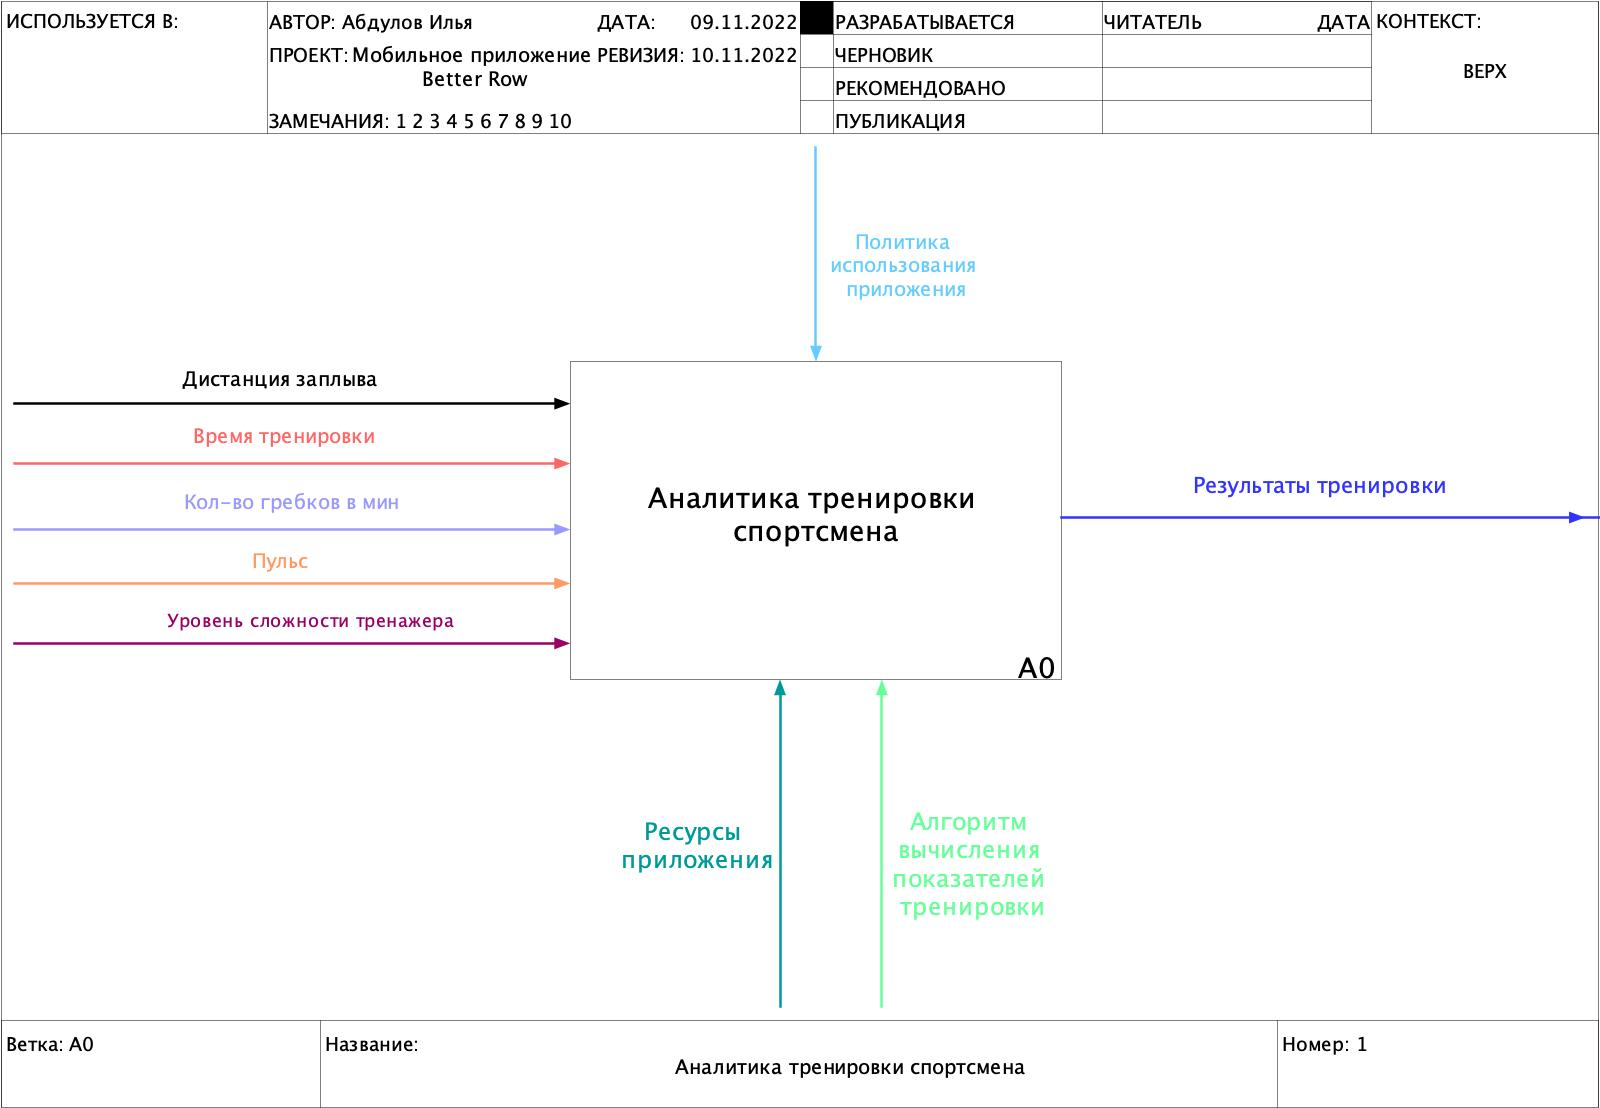
\includegraphics[width=1\linewidth]{01_A0.jpg}}
\caption{Функциональная модель в стандарте IDEF0}
\label{fig11}
\end{figure}

\begin{figure}[H]
\centerline{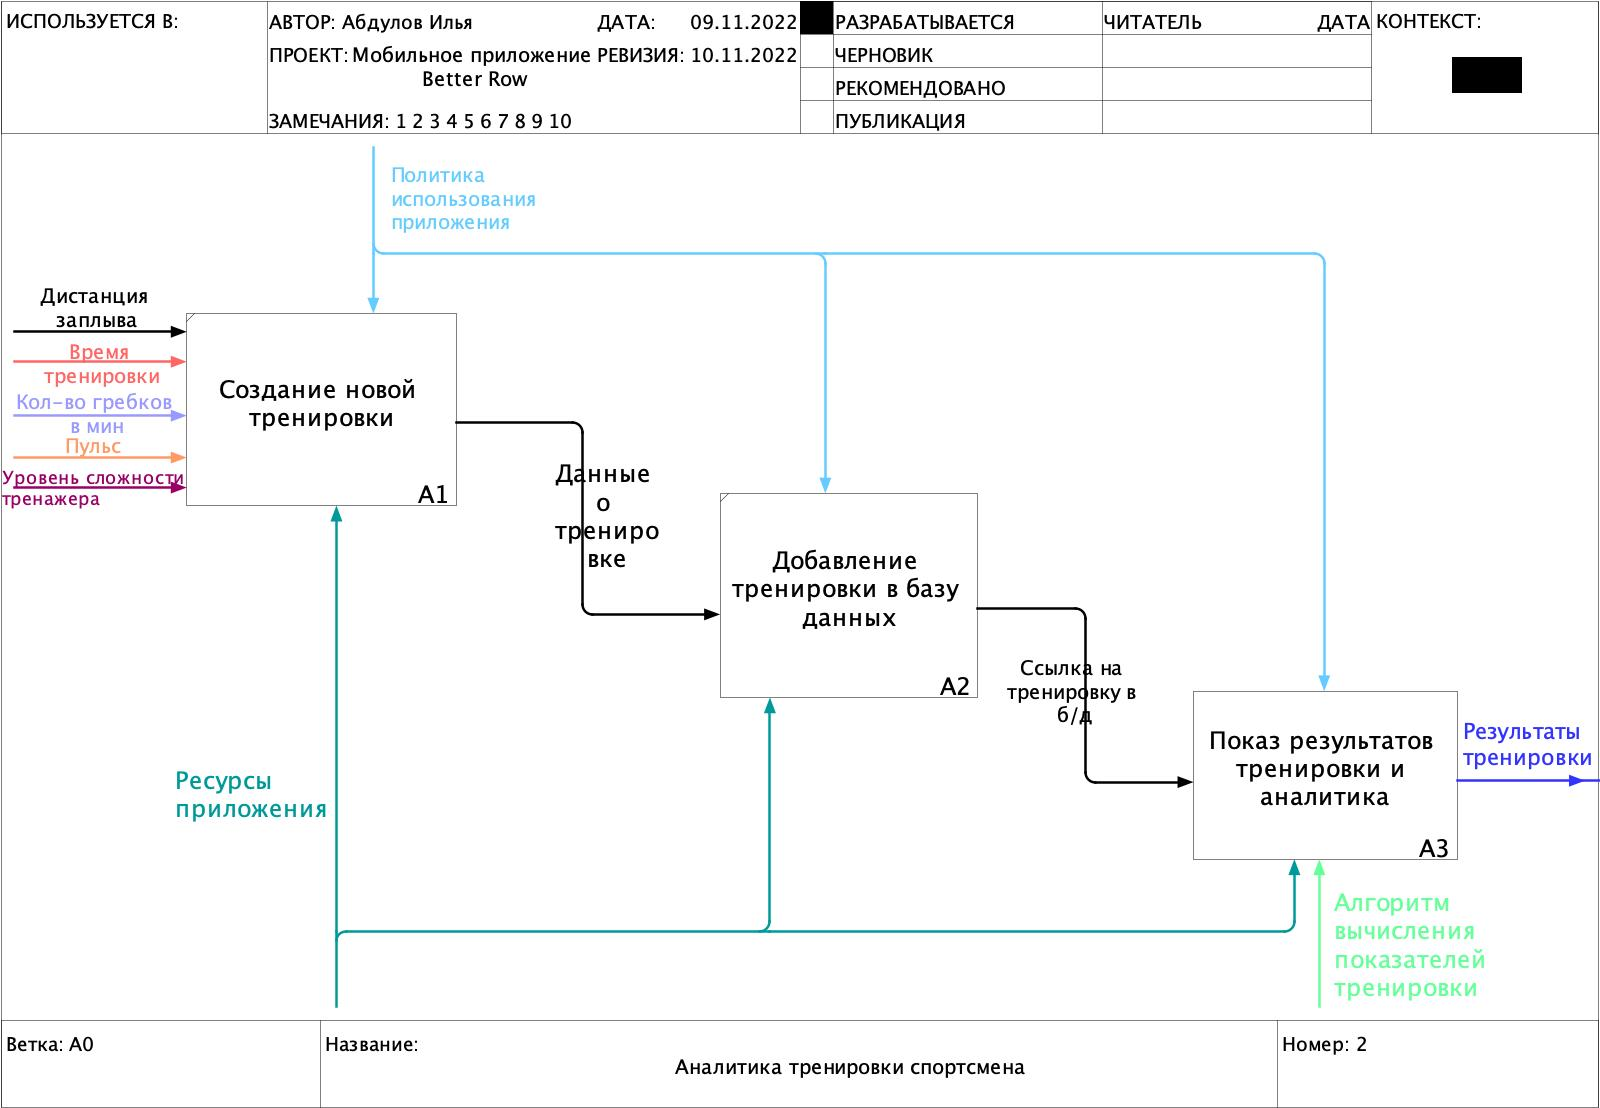
\includegraphics[width=1\linewidth]{02_A0.jpg}}
\caption{Первый уровень декомпозиции "Аналитика тренировки спортсмена"}
\label{fig12}
\end{figure}

\begin{figure}[H]
\centerline{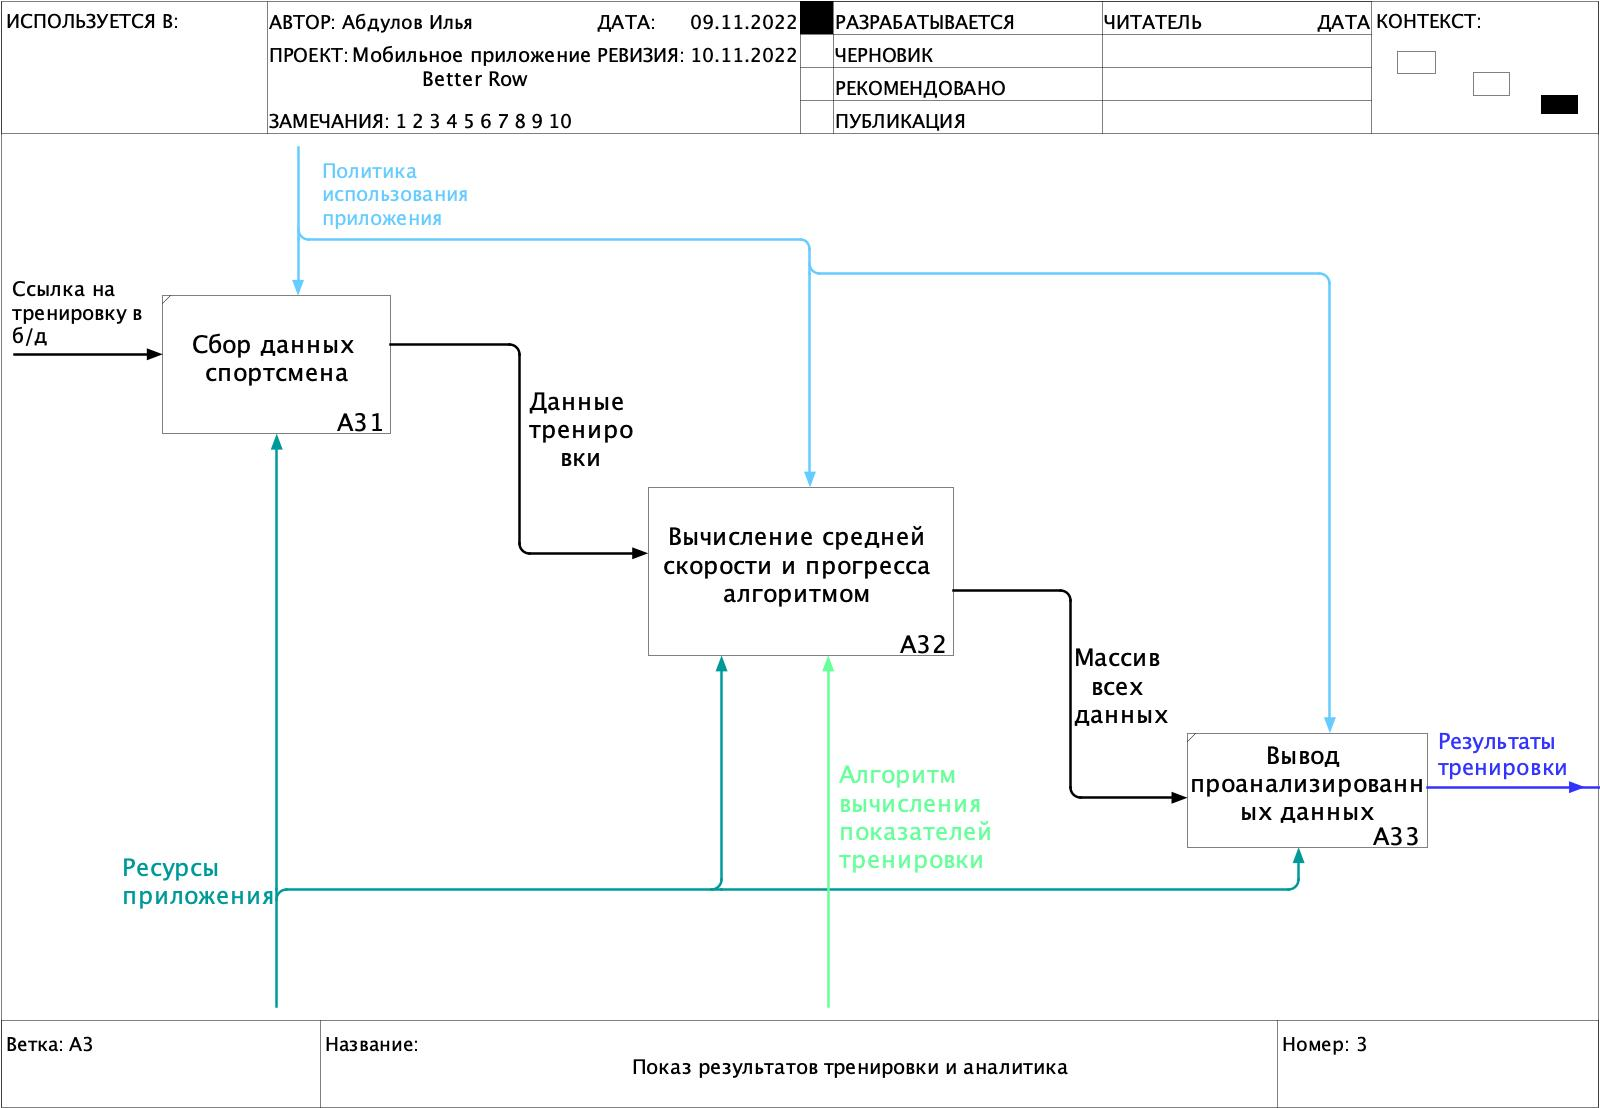
\includegraphics[width=1\linewidth]{03_A3.jpg}}
\caption{Второй уровень декомпозиции "Показ результатов тренировки и аналитика"}
\label{fig13}
\end{figure}

\begin{figure}[H]
\centerline{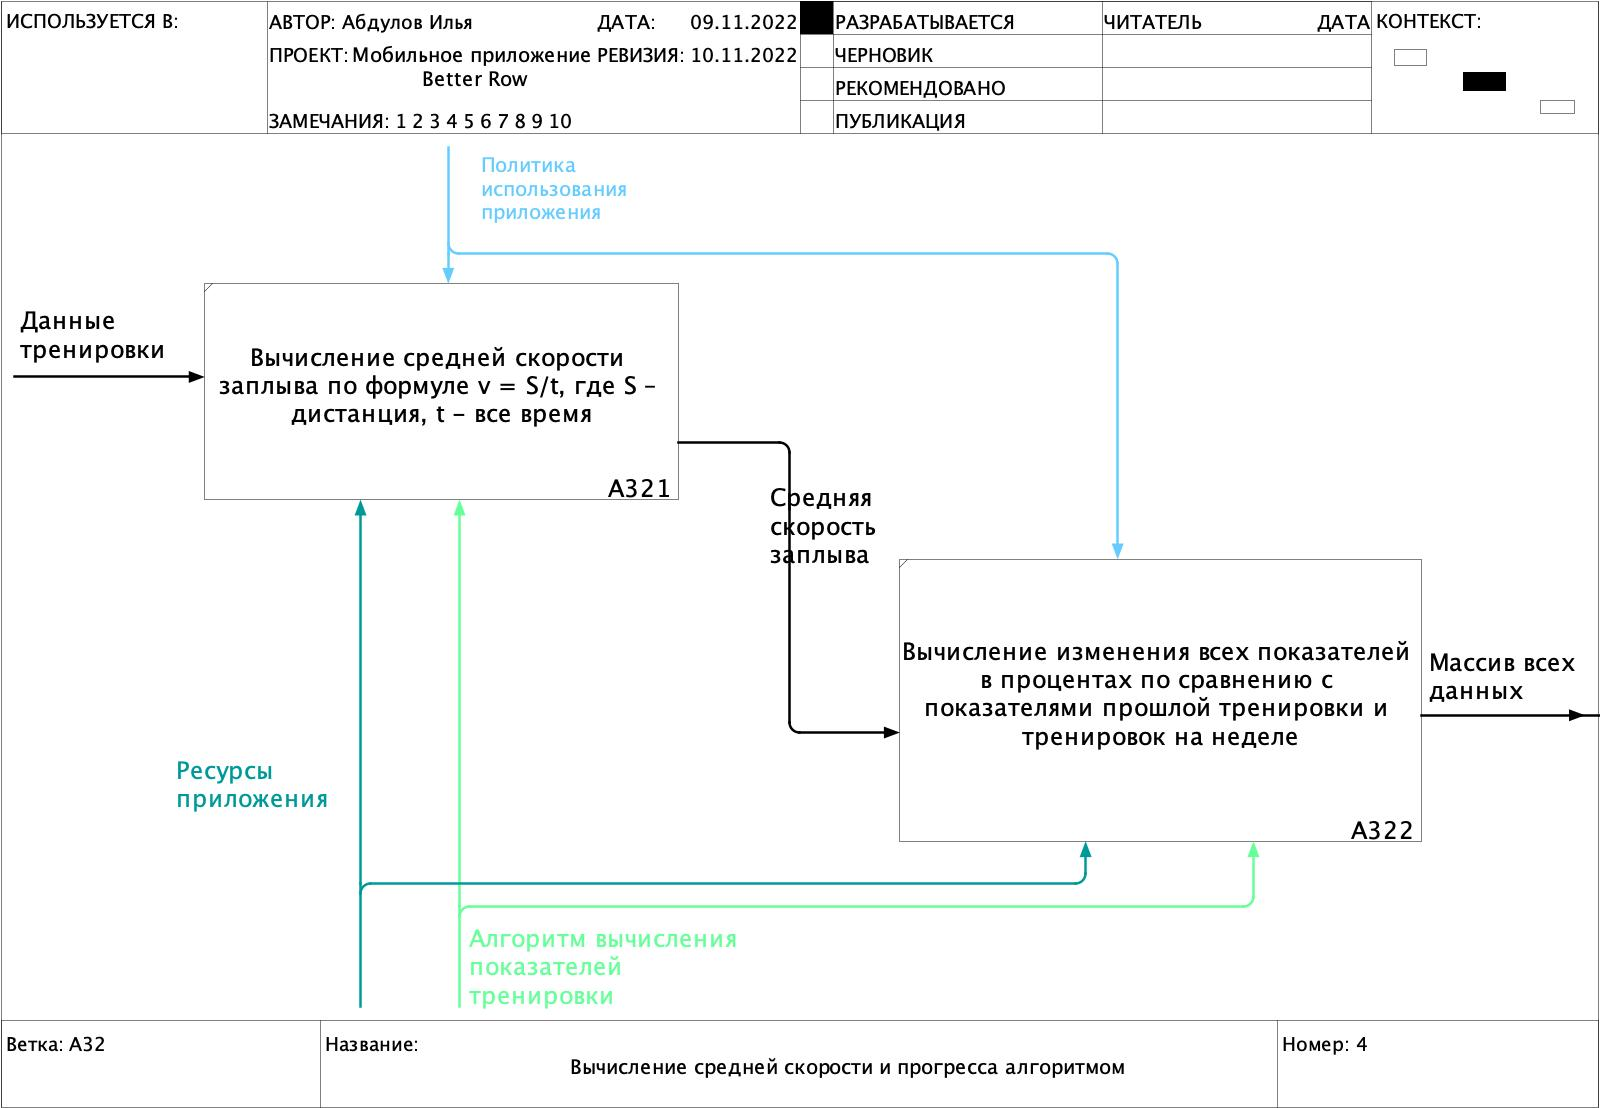
\includegraphics[width=1\linewidth]{04_A32.jpg}}
\caption{Третий уровень декомпозиции "Вычисление средней скорости и прогресса алгоритмом"}
\label{fig14}
\end{figure}

Предусмотрено наличие обратных связей между работами по входу или управлению. В функциональной модели и декомпозициях обратных связей нет.

\begin{landscape}

\subsection{Диаграммы DFD}
\begin{figure}[H]
\centerline{\includegraphics[width=0.73\linewidth]{A-0_DFD_diagram.pdf}}
\caption{Контекстная диаграмма в стандарте DFD}
\label{fig11}
\end{figure}

\begin{figure}[H]
\centerline{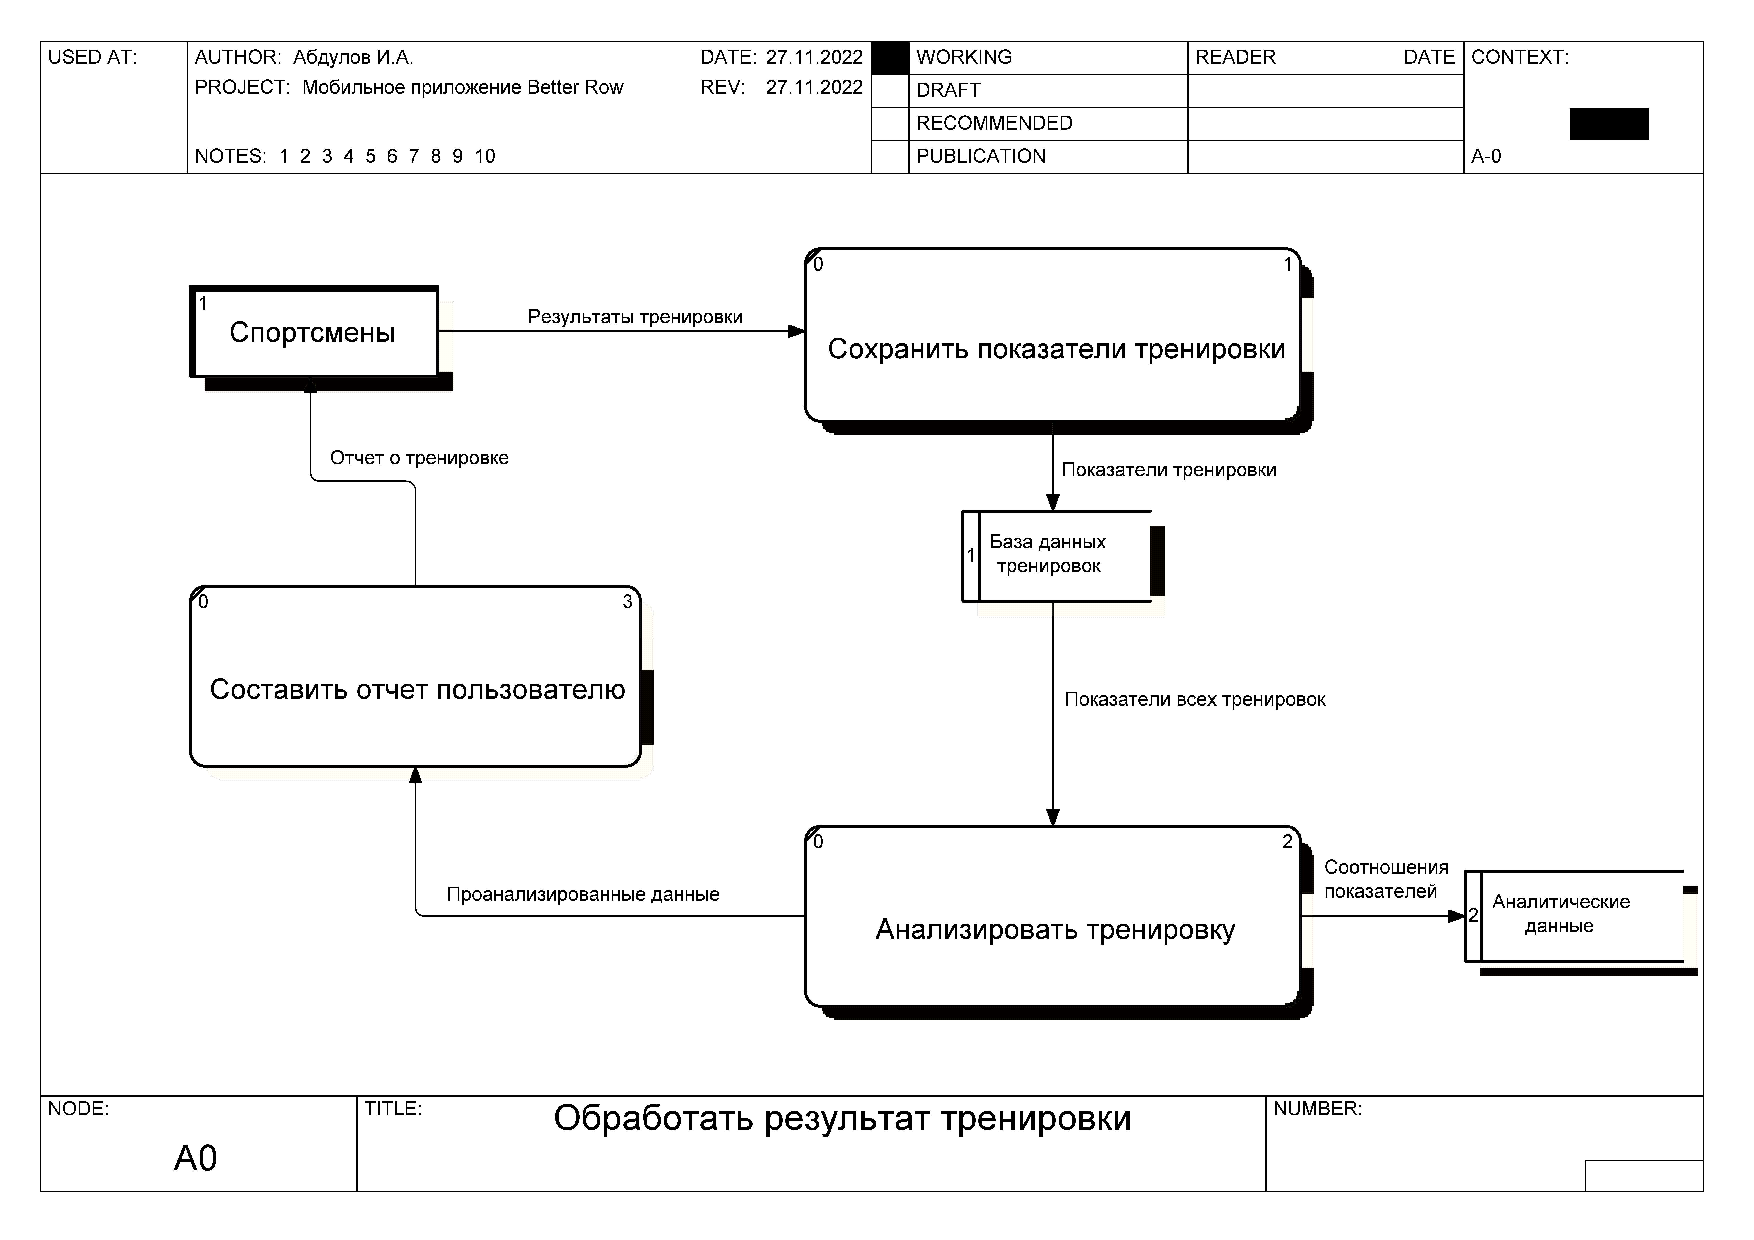
\includegraphics[width=0.8\linewidth]{A0_DFD_diagram.pdf}}
\caption{Декомпозиция блока "Обработать результат тренировки"{} в стандарте DFD}
\label{fig12}
\end{figure}

\subsection{Модель IDEF3}

\begin{figure}[H]
\centerline{\includegraphics[width=0.73\linewidth]{01_IDEF3.pdf}}
\caption{Блок "Система работы приложения"{} в IDEF3}
\label{fig13}
\end{figure}

\begin{figure}[H]
\centerline{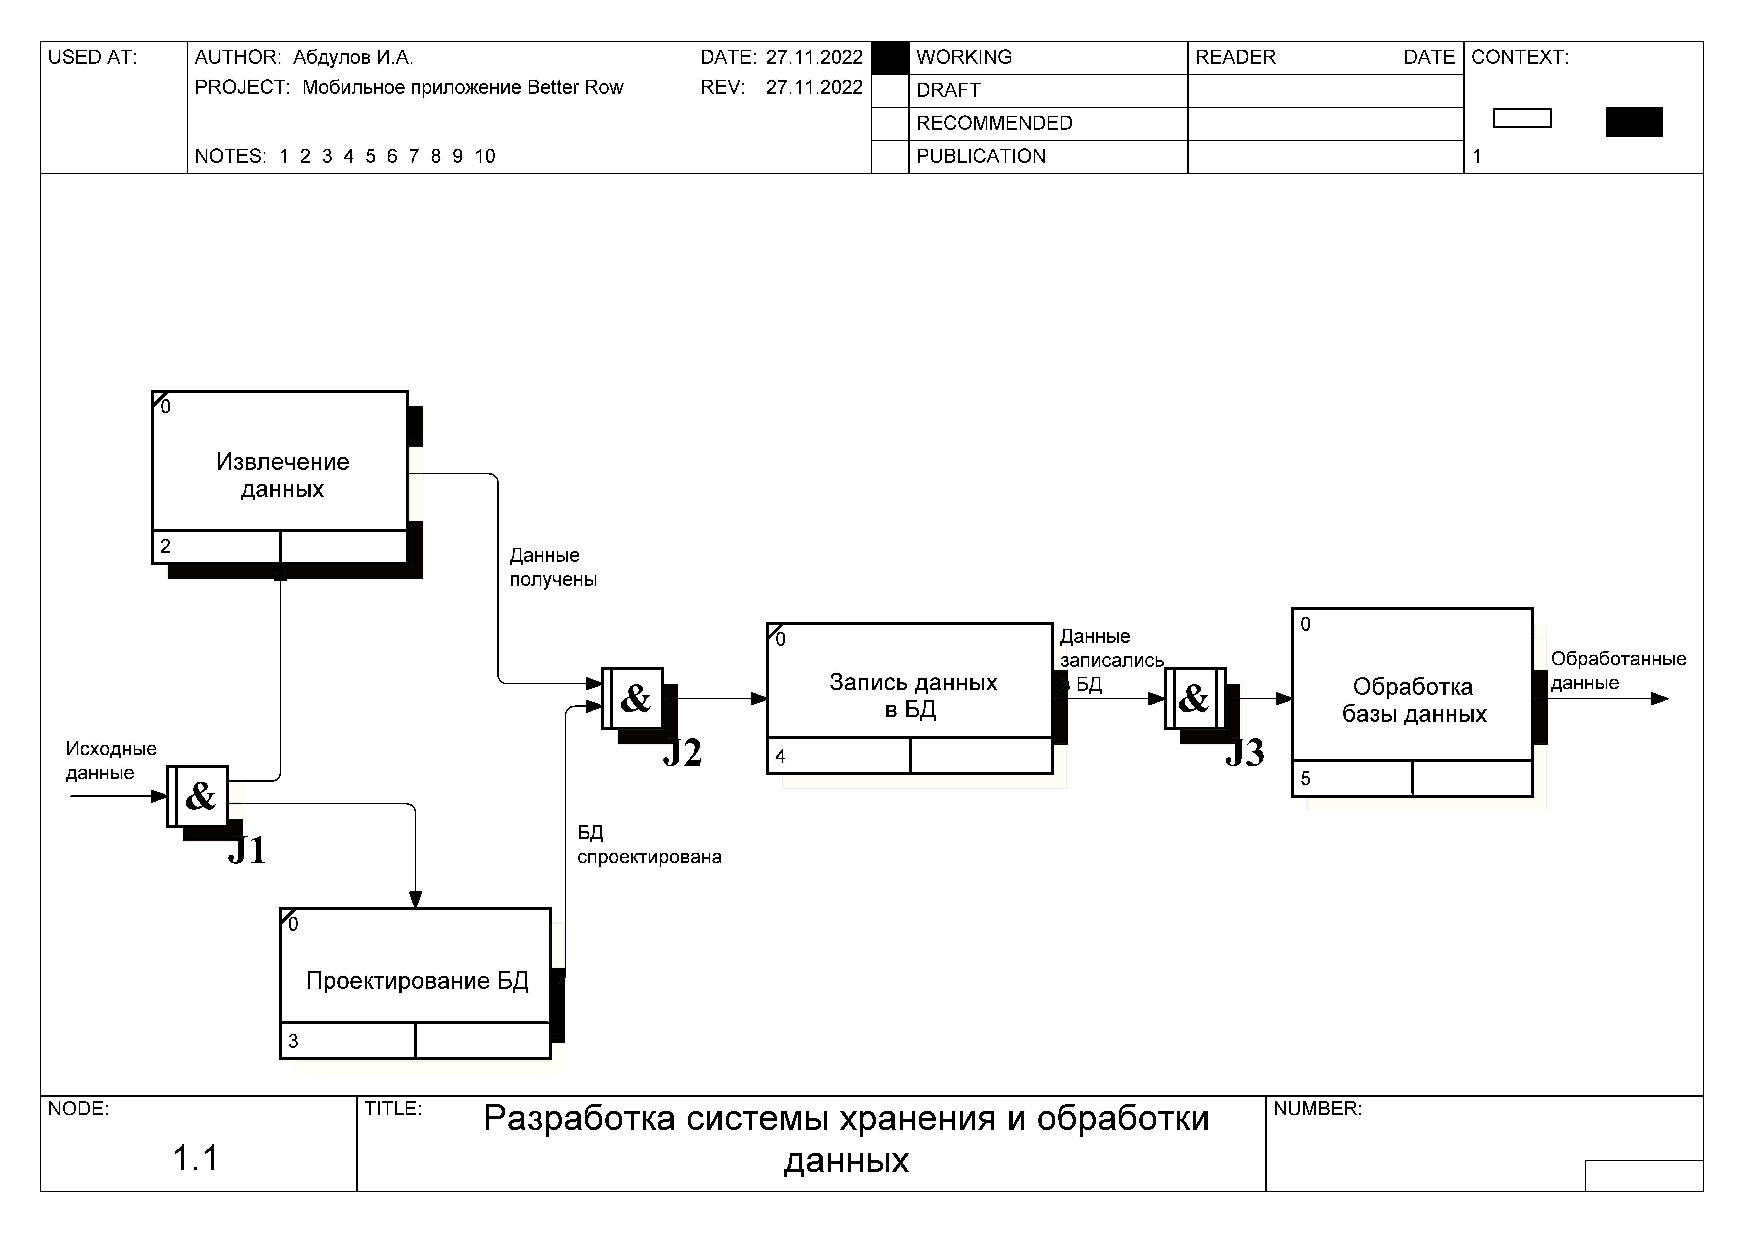
\includegraphics[width=0.8\linewidth]{1-1_IDEF3.pdf}}
\caption{Декомпозиция блока "Разработка системы хранения и обработки данных"{} в IDEF3}
\label{fig14}
\end{figure}

\begin{figure}[H]
\centerline{\includegraphics[width=0.8\linewidth]{5-1_IDEF3.pdf}}
\caption{Декомпозиция блока "Обработка базы данных"{} в IDEF3}
\label{fig15}
\end{figure}

\end{landscape}



\chapter{Создание технического задания на создание информационной системы.}

\section{Общие сведения}

\subsection{Наименование работ}

Выполнение в 2022 году работ по созданию информационной системы для спортивного клуба по академической гребле "Rowing Club"\ университета ИТМО.

\subsection{Плановые сроки выполнения работ}

В течение 75 дней с даты заключения договора с клубом по академической гребле университета ИТМО. Сроки создания информационной системы должны соответствовать календарному плану.

\subsection{Цели и задачи выполнения работ}

Основной целью выполнения работ является повышение уровня подготовки спортсменов по дисциплине гребля к межвузовским соревнованиям.

Выполняемые работы направлены на решение следующих задач:

\begin{itemize}
\item повышение уровня подготовки спортсменов к межвузовским соревнованием;
\item создание информационной системы клуба академической гребли "ITMO Rowing Club";
\item построение единой системы, содержащей всех гребцов университета ИТМО с их спортивными данными и показателями.
\end{itemize}

\subsection{Основные направления выполнения работ}

В рамках работ производится создание спортивного вузовского мобильного приложения, обеспечивающего процесс записи и анализа показателей спортсменов гребцов для отслеживания их прогресса.

\section{Общие требования к системе}

\subsection{Требования по сохранности информации при авариях}

Сохранность информации в развиваемой системе должна обеспечиваться при разрушении данных при механических и электронных сбоях и
отказах в работе компьютеров: на основе программных процедур
восстановления информации с использованием хранимых копий баз данных,
программных файлов системы, а также загружаемых файлов.

Система должна восстанавливаться при перезапуске аппаратных средств.

Для обеспечения сохранности информации в Системе должны быть
включены следующие функции:
\begin{itemize}
\item резервное копирование операционных систем, баз данных,
программных и загружаемых файлов;
\item восстановление данных в непротиворечивое состояние при
программно-аппаратных сбоях (отключение электрического питания, сбоях
операционной системы и других) вычислительно-операционной среды
функционирования;
\item	восстановление данных в непротиворечивое состояние при сбоях в
работе сетевого программного и аппаратного обеспечения.
\end{itemize}

\subsection{Требования к надежности}

Спроектированные архитектурные решения системы должны быть
устойчивы по отношению к программно-аппаратным ошибкам, отказам
технических и программных средств, с возможностью восстановления ее
работоспособности и целостности информационного содержимого при
возникновении ошибок и отказов.

\subsection{Требования к режимам функционирования}

Система должна иметь возможность функционировать в двух
режимах: штатном и режиме системного администрирования.

Штатный режим должен являться основным режимом
функционирования, обеспечивающим выполнение задач системы.

Режим системного администрирования должен являться технологическим
режимом и использоваться для сопровождения системы, в том числе –
изменения конфигурации, параметров работы, настроек, выполнения
регламентного обслуживания программно-технических средств. Кроме этого, в
режиме системного администрирования должны выполняться функции,
связанные с реконфигурацией, конвертированием и архивированием баз
данных системы. После возникновения отказа в каком-либо из компонентов
системы, режим должен обеспечивать перевод отказавших компонентов в
штатный режим функционирования после идентификации возникшего отказа и
устранения его причин.

\section{Создание информационной системы}

\subsection{Полное наименование системы}

Полное наименование: мобильное приложение Better Row.

Условное обозначение: Better Row.

\subsection{Цель работы}

Целью настоящей работы является создание мобильного приложения для развития спортивной деятельности в университете ИТМО, информационная система разрабатывается для клуба по академической гребле.

\subsection{Характеристика объекта автоматизации}

Объектами автоматизации являются процессы по управлению информационной системой, а также контроль эффективности работы программного обеспечения системы. 

Пользователями системы являются:
\begin{itemize}
\item руководство университета ИТМО;
\item руководство и представители гребного клуба университета;
\item участники гребного клуба университета;
\item персонал системы (администраторы).
\end{itemize}

Жалобы на эффективность работы информационной системы могут быть поданы:
\begin{itemize}
\item посредством портала системы;
\item по почте;
\item по мобильному телефону, указанным исполнителем в договоре.
\end{itemize}

\subsection{Требования к системе в целом}

Информационная система должна:
\begin{itemize}
\item упростить отслеживание тренировок;
\item сохранять записи о результатах тренировок;
\item отслеживать спортивный прогресс;
\item создавать аналитику по результатам тренировок.
\end{itemize}

\subsection{Требования к функциональной части системы}

Мобильное приложение Better Row должно состоять из:
\begin{itemize}
\item главного раздела, откуда осуществляется переход к основным подразделам приложения;
\item подраздела результатов и статистики, где отображаются добавленные тренировки по датам, и где можно добавить данные о новой тренировке;
\item подраздела расписания, где отображаются даты тренировок спортивного клуба;
\item подраздела настроек приложения, содержащего справочную и статистическую
информацию о приложении;
\item ЛК тренера или другого руководящего лица, обеспечивающий просмотр информации о результатах и прогрессе спортсменов;
\item ЛК спортсмена, обеспечивающий просмотр своих персональных данных.
\end{itemize}

Портал системы должен обеспечивать спортсмену:
\begin{itemize}
\item возможность внесения данных и показателей тренировки;
\item возможность сохранить результаты тренировки;
\item возможность удалить запись тренировки;
\item возможность просмотреть статистику тренировок;
\item возможность просмотреть прогресс тренировок. 
\end{itemize}

Портал системы должен обеспечивать руководству:
\begin{itemize}
\item возможность просмотреть список всех спортсменов в клубе;
\item возможность просмотреть статистику тренировок выбранного спортсмена;
\item возможность просмотреть прогресс спортсмена;
\item возможность удалить выбранного спортсмена из базы данных спортсменов.
\end{itemize}

Интерактивная форма внесения результатов тренировки должна обеспечивать внесение следующей информации:
\begin{itemize}
\item дистанция заплыва;
\item время заплыва;
\item темп заплыва;
\item пульс спортсмена.
\end{itemize}

Полученная информация о результате тренировки спортсмена должна размещаться в соответствующем подразделе результатов и статистики после прохождения формально-логической проверки автоматически сразу после поступления информации в систему. Автоматизированная формально-логическая проверка должна предусматривать проверку правильности заполнения интерактивных форм и полей ввода данных. В случае отрицательного результата проверки информация не должна вноситься в базу данных, лицо,
представившее информацию в систему, должно извещаться об этом
посредством системы и ему должна быть предоставлена возможность повторно
представить информацию в систему для внесения в базу данных с учетом
необходимых исправлений.

Система должна обеспечивать оперативное хранение записей тренировок спортсменов в течении 3 (трех) лет с момента их размещения в системе. По истечении указанного срока хранения информации о показателях тренировок спортсменов средствами СУБД предоставляет возможность выполнить её архивирование с возможностью доступа к ней администраторам системы.

В системе должна быть обеспечена возможность для руководства гребного клуба автоматической
выгрузки во внешнюю информационную среду информации по тренировкам спортсменов из мобильного приложения в виде электронной таблицы для удобной работы с большим количеством результатов и создания общепринятой отчетности.

\subsection{Требования к видам обеспечения}

Специальных требований к математическому обеспечению не
предъявляется. Специальные алгоритмы должны быть разработаны на стадии
технического проектирования.

Требования к информационному обеспечению определяются
функциональностью системы.

Графический пользовательский интерфейс должен быть реализован как
мобильное приложение, используемое пользователями через мобильные устройства на операционной системе IOS, Android, ChromeOS версий, официально поддерживаемых производителями.

Макеты визуализации и дизайна форм системы должны быть разработаны и
представлены на этапе технического проектирования.

В ходе выполнения работ в рамках данного технического задания должна
быть создана рабочая группа по управлению ходом работ, в состав которой
должны входить представители гребного клуба и исполнителя. Регламент взаимодействия представителей должен определяться в рабочем порядке.

\subsection{Проведение испытаний}

Испытания должны осуществляться в соответствии с этапами работ,
определенными в календарном плане, являющимся приложением к настоящему
техническому заданию, и оформляться в соответствии с требованиями,
приведенными в разделе «Требования к документированию» настоящего
документа.

Для системы должны быть проведены следующие работы:
\begin{itemize}
\item предварительные комплексные испытания;
\item опытная эксплуатация;
\item приемочные испытания.
\end{itemize}

Испытания должны проводиться комиссией, состоящей из
уполномоченных представителей сторон приема и исполнения работ.

Испытания должны проводиться с учетом требований ГОСТ 34.603-92
«Виды испытаний автоматизированных систем».

Проверка выполнения требований функционального назначения системы
должна осуществляться на заданном в качестве контрольного примера наборе
данных в пределах функций системы, указанных в настоящем документе, а
также уточняющих его технических требованиях к отдельным компонентам
системы, разработанных на этапе технического проектирования.

При обнаружении дефектов испытываемого программного обеспечения
список дефектов фиксируется, после чего комиссией утверждается срок
исправления дефектов и дата повторного проведения испытаний.

\section{Требования к результатам работ}

\subsection{Разработка прикладного программного обеспечения}

В ходе разработки прикладного программного обеспечения должны быть
выполнены следующие работы:
\begin{itemize}
\item разработка прикладного программного обеспечения согласно
требованиям настоящего технического задания;
\item установка и настройка прикладного программного обеспечения на
подготовленные технические средства, с установленным и настроенным
системным программным обеспечением. Технические средства для
демонстрации системы предоставляются исполнителем;
\item оформление исходных текстов прикладного программного обеспечения
и программной документации согласно требованиям настоящего
технического задания.
\end{itemize}

\subsection{Требования к составу и содержанию работ по подготовке объекта автоматизации к вводу системы в действие}

Система при вводе её в эксплуатацию должна пройти предварительные
комплексные испытания, опытную эксплуатацию и приемочные испытания.

Приемочным испытаниям системы должна предшествовать ее опытная
эксплуатация.

Исполнитель должен обеспечить функционирование системы в период
опытной эксплуатации на мощностях, определяемых гребным клубом.

В ходе подготовки объекта автоматизации к вводу системы в действие
должна быть произведена инсталляция общесистемного и прикладного программного
обеспечения. Инсталляция прикладного программного обеспечения должна
осуществляться в соответствии с руководством системного администратора со стороны исполнителя.

\section{Требования к документированию}

\subsection{Требования к оформлению}

Отчетная документация должна прилагаться в бумажном и электронном
виде (на оптическом CD или DVD или USB носителе) на русском языке.

Вспомогательная документация (не указанная в качестве непосредственного
результата работ) передается только в электронном виде.

Для каждого этапа должен быть представлен краткий отчет в форме
презентации.

\subsection{Проектная и рабочая документация}

Проектная и рабочая документация должна разрабатываться с учетом
требований комплекса государственных стандартов «Информационная
технология. Комплекс стандартов на автоматизированные системы»:
\begin{itemize}
\item ГОСТ 34.601-90 «Автоматизированные системы. Стадии создания»;
\item ГОСТ 34.003-90 «Автоматизированные системы. Термины и
определения»;
\item ГОСТ 34.602-89 «Техническое задание на создание
автоматизированной системы»;
\item ГОСТ 34.201-89 «Виды, комплектность и обозначение документов при
создании автоматизированных систем»;
\item ГОСТ 34.603-92 «Виды испытаний автоматизированных систем»;
\item РД 50-34.698-90 «Автоматизированные системы. Требования к
содержанию документов»;
\item ГОСТ 19.301-79 «Программа и методика испытаний. Требования к
содержанию и оформлению»;
\item ГОСТ 2.601-2006 «ЕСКД. Эксплуатационные документы»;
\item ГОСТ 2.106-96 «ЕСКД. Текстовые документы» (с изменениями от 22
июня 2006 года);
\item ГОСТ 2.120-73 «ЕСКД. Технический проект» (с изменениями от 22
июня 2006 года).
\end{itemize}

\subsection{Исходные тексты и программная документация}

Для каждой разрабатываемой системы должны быть представлены в
электронном виде (на оптическом CD или DVD или USB носителе):
\begin{itemize}
\item исходные тексты прикладного программного обеспечения, включая
контрольные суммы для каждого файла по алгоритму MD5;
\item инструкция по сборке из исходных текстов рабочего прикладного
программного обеспечения;
\item исполняемые файлы (где применимо), включая контрольные суммы
для каждого файла по алгоритму MD5;
\item описание программных средств, содержащее сведения об их
логической структуре и среде функционирования, а также описание методов,
приемов и правил эксплуатации технологических средств, используемых при
их создании;
\item описание применения, содержащее сведения о назначении
программных средств, области применения, применяемых методах, классе
решаемых задач, ограничениях при применении, минимальной конфигурации
технических средств, среде функционирования и порядке работы.
\end{itemize}

\subsection{Требования к оформлению документации по испытаниям системы}

Испытания развиваемой/создаваемой системы должны проводиться с
учетом требований ГОСТ 34.603-92 «Виды испытаний автоматизированных
систем».

\section{Источники разработки технического задания}

\subsection{Источники разработки}

Исходными документами для разработки данного технического задания и автоматизированной системы являются: материалы аналитического проектного исследования объекта автоматизации, действующие законодательные и нормативные правовые акты, в рамках которых функционирует объект автоматизации, нормативно-техническая документация, ГОСТ 34.602-89, образцы рабочих документов, полученных в процессе исследования, информационные материалы и проектная документация на аналогичные автоматизированные системы.

\conclusions

Цель работы была достигнута.

Было дано широкое описание будущего мобильного приложения. В отчёте были указаны: название, назначение, основные пользователи системы, планируемый набор функций для будущих пользователей, прототип интерфейса будущей системы, обзор аналогов на рынке и обоснование необходимости разработки системы.

Была описана предметная область функционирования, представлены пользователи будущего мобильного приложения. В отчёте были представлены диаграммы вариантов использования, активности для ключевых прецедентов и рассмотрены альтернативные потоки событий.

Были представлены построенные функциональные модели IDEF0, которые содержат 3 уровня декомпозиции,  диаграммы потоков данных DFD и модели IDEF3 с двумя уровнями декомпозиции.

Техническое задание на разработку информационной системы «Better Row» составлено. Составление технического задания на мобильное приложение является важным этапом разработки информационной системы. Правильно составленное ТЗ помогает:
\begin{enumerate}
\item увеличить шансы создать продукт, соответствующий задачам бизнеса;
\item подготовить точный прогноз относительно сроков и стоимости разработки;
\item избежать конфликтов между исполнителем и заказчиком из-за разного понимания задач и методов решения;
\item сократить риски изменений проекта из-за нечетко прописанных требований.
\end{enumerate}

Необходимо отметить, что при написании курсовой работы был получен опыт создания моделей и диаграмм в различных стандартах, а также получен опыт создания технического задания на информационную систему, что поможет при дальнейшей реализации и развития мобильного приложения «Better Row».

\newpage
\begin{thebibliography}{99}

\bibitem{bib1}Примеры технических заданий, составленных для аналогичных проектов — URL: \url{https://drive.google.com/drive/folders/1XbbDN72k7BuWoNRZJvKtHSEjfunnMn7w} (дата обращения 14.12.2022).

\bibitem{bib2}Комплекс стандартов на создание технического задания для автоматизированных систем ГОСТ 34.602-89 — URL: \url{https://drive.google.com/drive/folders/1L2nVVB2jm_JoFxdwLdpV8nnh6FVtEjEo} (дата обращения 14.12.2022).

\bibitem{bib3}Интернет-статья "Как написать ТЗ для мобильного приложения?"\ — URL: \url{https://sibdev.pro/blog/articles/kak-napisat-tz-dlya-mobilnogo-prilozheniya} (дата обращения 12.12.2022).

\bibitem{bib4}Интернет-статья "Разработка мобильного приложения: как написать техническое задание?"\ — URL: \url{https://sandev.ru/razrabotka-mobilnogo-prilozheniya-kak-napisat-tehnicheskoe-zadanie/} (дата обращения 14.12.2022).

\bibitem{bib5}Видео-лекция "ГОСТ 34 в современной разработке"\  — URL: \url{https://www.youtube.com/watch?v=Cb7oyeIjWZ8} (дата обращения 14.12.2022).

\bibitem{bib6}Интернет-сервис, который помогает создать прототипы интерфейсов ИС — URL: \url{https://www.figma.com/} (дата обращения 14.12.2022).	

\bibitem{bib7}Приложение StarUML для создания UML диаграмм — URL: \url{https://staruml.io/} (дата обращения 03.12.2022).	

\bibitem{bib8}Документация к StarUML — URL: \url{https://docs.staruml.io/} (дата обращения 02.12.2022).	

\bibitem{bib9}Интернет-статья по диаграммам вариантов использования в языке UML — URL: \url{http://sp.cs.msu.ru/ooap/exerb2019.html} (дата обращения 03.12.2022).	

\bibitem{bib10}Приложение Ramus для построения IDEF0 моделей — URL: \url{http://ramussoftware.com/} (дата обращения 09.12.2022).	

\bibitem{bib11}Интернет-статья по методологии IDEF0 — URL: \url{https://trinion.org/blog/idef0-znakomstvo-s-notaciey-i-primer-ispolzovaniya} (дата обращения 09.12.2022).	

\bibitem{bib12}Интернет-статья по построению диаграмм DFD — URL: \url{https://itteach.ru/bpwin/dfd-i-workflow-idef3} (дата обращения 26.11.2022).	

\bibitem{bib13}Интернет-статья по методологии IDEF3 — URL: \url{https://itteach.ru/bpwin/metodologiya-idef3} (дата обращения 26.11.2022).	

\bibitem{bib14}Интернет-приложение для создания моделей процессов BPMN — URL: \url{https://stormbpmn.com/} (дата обращения 27.11.2022).	
	
	
\end{thebibliography}

\end{document}
